\chapter{Background Information (optional)}
\label{chap:background}
A brief section giving background information may be necessary, especially if
your work spans two or more traditional fields. That means that your readers
may not have any experience with some of the material needed to follow your
thesis, so you need to give it to them. A different title than that given
above is usually better; e.g., "A Brief Review of Frammis Algebra." 

\section{A note from the template-author}
In a master thesis you might not need a background chapter. Discuss with your
advisor, whether it is feasible to put background information either in the
introduction or related-work chapter.

\section{An example of a TikZ image within text}
This section just demonstrates a coustom-macro for placing figures in the
text. The source-code for this macro is found in the file '\texttt{macros.tex}'.
Here is a reference to figure \ref{fig:figure-label2} on the next page.

\Blindtext

\FIG[The caption for the List-of-Figures]{The slightly longer caption,
containing additional information for the figure itself.}%
{figure-label2}{htbp}{%
    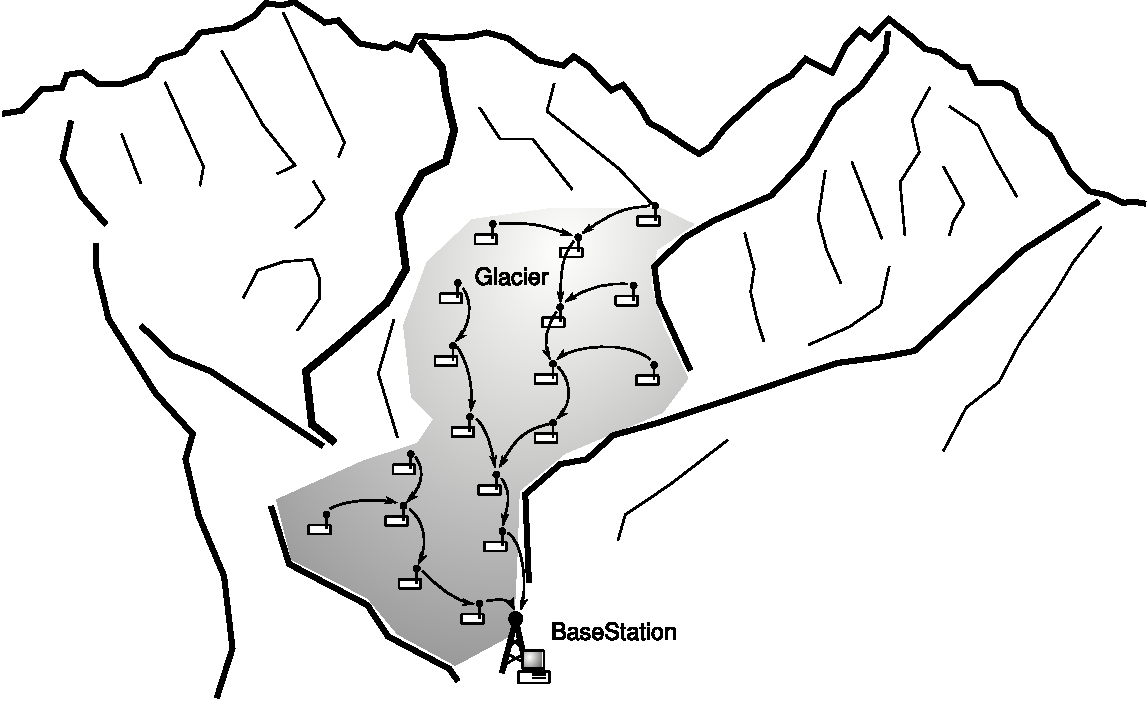
\includegraphics[width=0.8\linewidth]{img/Glacier.pdf}
}

\blindtext
\blinditemize

% vim: set ft=tex
